\RequirePackage{kvoptions-patch}
\documentclass[11pt,twoside]{scrartcl}
%\usepackage[ngerman]{babel}
\usepackage[T1]{fontenc}
\usepackage[utf8]{inputenc}
\usepackage{url}
\usepackage{lmodern}
\usepackage{amsmath}
\usepackage{graphicx}
\usepackage[
	title={Development of a FEM code for fluid-structure coupling},
	author={Stephan Herb},
	type=master,
	institute=ipvs,
	number=314159, %TODO Nummer vom Prüfungsamt/-ausschuss erfahren
	course=cs,
	examiner={Prof.\ Dr.\ Miriam Mehl},
	supervisor={Dipl.-Ing.\ Florian Lindner},
	startdate={2015-06-08},
	enddate={2015-12-08},
	crk={}, %TODO CRK-Klassifikation auf meine Arbeit ändern
	language=german
	]{uni-stuttgart-cs-cover}

\begin{document}
\Coverpage
\tableofcontents
\section{Introduction}
Here comes the introduction. And before that the abstract (that needs to be put into LaTeX as special paragraph)\newpage %TODO abstract-format in LaTeX irgendwie reinbringen
\section{Framework Evaluation}
Part of the thesis was to find several frameworks which ease the work with the finite element method. An evaluation of these frameworks was done to select a suitable one for the given task. The evaluation's criteria are presented in this chapter as well as a short description of the studied frameworks.
 \subsection{General Aspects}
In preparation of evaluating the frameworks many criteria were created to objectify the search for the most suitable. The individual aspects were as follows:
 \begin{itemize}
 \item Open Source: All frameworks under consideration need to be published under the GNU Lesser General Public License or similar license that allows modification and/or redistribution.
 \item Parallelization: In order to accelerate the calculations the framework has to be able to support the widely used Message Passing Interface (MPI).
 \item The programming language was chosen to be C++. Therefore the framework has to be written in this language. %TODO: warum c++: persönlich größere erfahrung, python wäre generell auch denkbar
 \item Mesh file import: Common mesh files types like gmsh or xda/xdr must be able to load by the framework. Simultaneously the framework must support finite elements like triangles and quadrilaterals with three and four nodes respectively and be able to handle two dimensional elements defined within three dimensional space. %TODO warum muss framework meshes importieren können, was setze ich beim mesh file voraus; es geht auch ein vom framework selbst definiertes format, so lange es die bedingungen erfüllt und einfach reproduzierbar ist
 \item The framework should handle different types of boundary conditions defined in a mesh file. %TODO diesen punkt mit dem vorigen verschmelzen, die bcs sind meine forderungen
 \item Built-in solvers: In order so solve the matrix-vector-system the framework must provide a variety of different iterative solvers. %TODO siehe zwischenvortrag: höhere flexibilität für anwender
 \item Convenience functions: To optimize the calculations the framework should make use of functions to get matrix-vector and matrix-matrix products, transpose matrix or sparse-matrices.
 \item Accessible and detailed documentation: In order to guarantee maintainability and expandability the framework has to have a good documentation itself. %TODO example-codes, dokumentierte klassen und funktionen, mailing-listen und/oder foren zur einfachen verständigung mit den entwicklern
 \item Up-to-date: The framework should be well maintained and actively supported by its developers to ensure a long term compatibility with possible new features of the thesis' code
 \item The framework should be used by at least a few projects. This shows the framework's importance and usability. %TODO nicht nur projects sondern auch publikationen
 \item Easy-to-learn syntax and structure: A rather subjective aspect but an important one. The limited time for the thesis does not allow to study highly complicated structures or semantics. This accompanies the documentation aspect.
 \end{itemize}
 \subsection{Frameworks Overview}
 The following list contains FEM libraries and frameworks which were evaluated.
%  \subsubsection{FEniCS}
  \subsubsection{Feel++}
  - "Feel++ is a unified C++ implementation of Galerkin methods (finite and spectral element methods) in 1D, 2D and 3D to solve partial differential equations."\cite{feelpp}\newline
  - creation of versatile mathematical kernels allow testing and comparing different techniques and methods in solving problems\newline
  - focus on close mathematical abstractions regarding partial differential equations (PDE)\newline
  - \cite{prud2012feel++}
  - imports e.g. gmsh mesh files\newline
  - seamlessly parallel with mpi\newline
  - currently used in projects at Cemosis (Center for Modeling and Simulation in Strasbourg, France) including fluid structure interactions, high field magnets simulation, or, optical tomography\newline
  - actively developed, last major release were on February 2015
  \subsubsection{OOFEM}\cite{oofem}
  - Object Oriented Finite Element Solver (OOFEM) 
  - actively developed with latest release from February 2014\newline
  - object oriented architecture; extensible in terms of new element types, boundary conditions or numerical algorithms\newline
  - modules for structural mechanics, transport problems and fluid dynamics\newline
  - focuses on efficient and robust solution to mechanical, transport and fluid problems\newline
  - written in C++ with focus on portability\newline
  - interfaces to various external software libraries like PETSc, ParMETIS, or, ParaView\newline
  - is used in several publications \cite{oofemPubs}
  \subsubsection{GetFEM++}
  - latest release from July 2015
  - framework for solving potentially coupled systems of linear and nonlinear PDE\newline
  - written in C++ but provides interfaces to languages like Python and Matlab\newline
  - model description that gather the variables, data and terms of a problem and some predefined bricks representing classical models\newline
  - easy switching from one method to another due to separation of geometric transformation, integration methods, and, finite element method\newline
  - can be used to construct generic finite element codes, where methods and the problem's dimension can be changed very easily\newline
  - uses MPI for parallelization, though it is stated that "a certain number of procedures are still remaining sequential" \cite{getfemppMPI}
  - imports e.g. gmsh mesh files\newline
  - used in project like IceTools \cite{icetools} (open source model for glaciers), EChem++ \cite{echempp} (Problem Solving Environment for Electochemistry) and SimNIBS \cite{simnibs} (software for Simulation of Non-invasive Brain Stimulation)
  \subsubsection{MFEM}\cite{mfem}
  - The Modular Finite Element Method (MFEM) library acts as a toolbox that provides the building blocks for developing finite element algorithms\newline
  - it has a wide range of mesh types, e.g. triangular and quadrilateral 2D elements, curved boundary elements or topologically periodic meshes\newline
  - supports MPI-based parallelism throughout the library\newline
  - variety of built-in solvers\newline
  - written in highly portable C++ and extensible due to separation of mesh, finite element and linear algebra abstractions\newline
  - hypre library is tightly integrated within MFEM, for example the use of high-performance preconditioners
  - The object oriented design of the library as well as the separation of the different parts of the library like the mesh functions, the finite elements, and, the linear algebra, focusing on adapt the code to a variety of applications
  - use in several publications \cite{mfemPubs}
  \subsubsection{libMesh}\cite{libmesh}
  - actively developed and active user community\newline
  - wide variety of mesh file formats to import from (e.g. gmsh, vtk, xda, )\newline
  - seamlessly integrated parallel functionality with MPI\newline
  - seamlessly interfaces optional external libraries like PETSc or ParMETIS\newline
  - complete documentation and documented source code available\newline
  - "framework for the numerical simulation of PDE using arbitrary unstructured discretizations on serial and parallel platforms".\newline
  - "provide support for adaptive mesh refinement (AMR) computations in parallel"\newline
  - supports a variety of 1D, 2D, and 3D geometric and finite element types\newline
  - created at The University of Texas at Austin in the CFDLab in March 2002. Contributions have come from developers at the Technische Universität Hamburg-Harburg Institute of Modelling and Computation, CFDLab associates at the PECOS Center at UT-Austin, the Computational Frameworks Group at Idaho National Laboratory, NASA Lyndon B. Johnson Space Center, and MIT.
% \subsection{Comparison}
\newpage
\section{Shell Elements}
Mathematical fundamentals of shell elements divided into the two parts and the coordinate transformation
 \subsection{Introduction to Linear Elasticity Problems}
 - \cite{steinke2005finite} ch3.1 (S.61)\newline
 - Einführung von Vektoren und Matrizen (Verschiebungsvektor, Tensoren bzw. Vektoren der Dehnungen und Spannungen)\newline
 - Verknüpfung der Versch. mit den Dehnungen + Stoffgesetz (kinematische Beziehung)\newline
 - ???
 
 In the following the fundamental equations of linear elasticity will be considered. Here, the spatial case is used for demonstration, but every lower dimensional problem can easily be derived from it.
 The following definitions will be used in this thesis:
 \begin{equation}
 \vec{u}^T = \left(u\ v\ w\right)\ \mathrm{displacement\ vector}
 \end{equation}
 \begin{equation}
 \vec{f}^T = \left(f_x\ f_y\ f_z\right)\ \mathrm{external\ force\ vector}
 \end{equation}
 The strains and stresses can either be described in form of tensors $\underline{\epsilon}$ and $\underline{\sigma}$, or as vectors $\vec{\epsilon}$ and $\vec{\sigma}$:
 \begin{equation}
 \underline{\epsilon} = \begin{pmatrix}
 \epsilon_{xx} & \epsilon_{xy} & \epsilon_{xz} \\
 \epsilon_{yx} & \epsilon_{yy} & \epsilon_{yz} \\
 \epsilon_{zx} & \epsilon_{zy} & \epsilon_{zz} \end{pmatrix};
 \underline{\sigma} = \begin{pmatrix}
 \sigma_{xx} & \sigma_{xy} & \sigma_{xz} \\
 \sigma_{yx} & \sigma_{yy} & \sigma_{yz} \\
 \sigma_{zx} & \sigma_{zy} & \sigma_{zz} \end{pmatrix}
 \end{equation}
 \begin{equation}
 \vec{\epsilon}^T = \begin{pmatrix}
 \epsilon_{xx} & \epsilon_{yy} & \epsilon_{zz} & 2\epsilon_{xy} & 2\epsilon_{yz} & 2\epsilon_{zx} \end{pmatrix};
 \vec{\sigma}^T = \begin{pmatrix}
 \sigma_{xx} & \sigma_{yy} & \sigma_{zz} & \sigma_{xy} & \sigma_{yz} & \sigma_{zx} \end{pmatrix}
 \end{equation}
 As stated in \cite{steinke2005finite} the relation between displacements and strains is as follows:
 \begin{equation}\label{eq:displ_strain_relation}
 \underline{\epsilon} = \frac{1}{2}\left(\nabla\vec{u} + \vec{u}\:\nabla \right);\quad \vec{\epsilon}
 %= \begin{pmatrix}
 %\frac{\partial}{\partial x} & 0 \\
 %0 & \frac{\partial}{\partial y} \\
 %\frac{\partial}{\partial y} & \frac{\partial}{\partial x} \end{pmatrix} \vec{u}
 = \underline{L}\vec{u}
 \end{equation}
 Equation \ref{eq:displ_strain_relation} relates the displacement vector field $\vec{u}$ with the strain field $\underline{\epsilon}$, or $\vec{\epsilon}$ respectively. Here, $\underline{L}$ is a differential operator. This strain-displacement relation is also called \textit{kinematic relationship} \cite{steinke2005finite}.\\
 In general initial strains can exist inside the material for example due to temperature changes or shrinkage. Such initial strains are denoted $\vec{\epsilon_0}$ and the stresses will be influenced by the difference between the actual and initial strains. Additionally one could imagine initial residual stresses $\vec{\sigma_0}$ that can be added to the general equation:
 \begin{equation}\label{eq:stress-strain-relation}
 \vec{\sigma} = \underline{D}\left(\vec{\epsilon}-\vec{\epsilon_0}\right)+\vec{\sigma_0},
 \end{equation}
 where $\underline{D}$ is the material matrix. In the simplest case of linear elasticity with isotropy, $\underline{D}$ only contains two parameters, namely the elastic modulus $E$ (also known as the Young's modulus) and the Poisson's ratio $\nu$. The former one defines the relationship between the stress and strain in a material, the latter one results as the quotient of the fraction of expansion and the fraction of compression for small changes.
 In the following the initial conditions are ignored, resulting in the a simpler form of equation \ref{eq:stress-strain-relation}:
 \begin{equation}
 \vec{\sigma} = \underline{D}\ \vec{\epsilon}
 \end{equation}
 For the said isotropic case $\underline{D}$ results in \cite{zienkiewicz2000finite}:
 \begin{equation}
 \underline{D} = \frac{E}{1-\nu^2}\begin{pmatrix}
 1 & \nu & 0 \\
 \nu & 1 & 0 \\
 0 & 0 & \frac{1-\nu}{2}
 \end{pmatrix}
 \end{equation}
 \subsection{Plane Element}
 First part of shell element: plane part. derivation of this part with two exemplary finite element types
  \subsubsection{Problem Definition}\label{sec:PlaneProbDef}
  %- Bild ähnlich ch7.1 mit xy-Ausdehnung, Dicke t, Mittelfläche, Rand, KoSys; Streckenlast q0 und Volumenkraft g aber weglassen\newline
  \begin{figure}
\centering
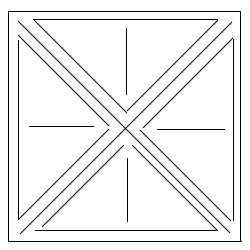
\includegraphics[width=0.7\linewidth]{figures/platzhalter}
\caption[kurze Unter-Überschrift]{lange Unter-Überschrift}
\label{fig:platzhalter}
\end{figure}
  In figure \ref{fig:platzhalter} an object is shown which extends to the x and y axis as its primary direction. The extend in z-direction is smaller and denoted by thickness $t$. The mid place located in between the top and bottom surface areas has the coordinate $z=0$. Its local z-axis equals the normal vector of the mid place. Such an object is called \textit{plane} in the following.
  
  %- Bed. für ebenen Spannungszustand (eb. Dehnungszustand erwähnen und auf Ref (z.B. Zienkiewicz) verweisen)\newline
  There are two different problem definitions regarding plane elements: Plane stress and plane strain. The directions of displacements $u$ and $v$ along the orthogonal local x and y axis defining its displacement field is a common feature of both problems. Also, both have in common, that only strains and stresses in the xy plane have to be considered: Instead of nine, only three components remain. While in the case of plane stress all other stress components are zero, in plane strain the stress in direction perpendicular to the xy plane is non-zero. In this thesis only plane stress will be discussed in further detail. More information about plane strain is given in \cite{zienkiewicz2000finite}. %TODO weitere referenz mit details dazu
  The following conditions must be satisfied such that a plane can be in \textit{plane stress} \cite{steinke2005finite}:
  \begin{itemize}
  	\item The thickness $t$ varies only slightly and it must hold: $t/l \ll 1$, with $l$ the extent of the larger side of the plane element.
  	\item The load is applied to the mid place.
  	\item Displacements, strains and stresses are constant across the thickness.
  \end{itemize}
  The stress components $\sigma_{xz},\sigma_{yz},\sigma_{zz}$ normal to the surface areas with $z \pm t/2$ vanish (equals zero). Therefore only the two normal stress components $\sigma_{xx}$ and $\sigma_{yy}$ and the transverse stress component $\sigma_{xy}$ are left non-zero.
    
  %- Verschiebungen, Dehnungen und Spannungen beschreiben + kinematische Beziehung + Stoffgleichung\newline
  Displacements can only occur in x and y direction. $u$ will be the displacement along x and $v$ along y. The displacement field $\vec{u}$ is as follows:
  \begin{equation}
  \vec{u}=\begin{pmatrix}
  u(x,y) & v(x,y)
  \end{pmatrix}^T
  \end{equation}
  The vector for the strain components:
  \begin{equation}
  \vec{\epsilon}=\begin{pmatrix}
  \epsilon_{xx} & \epsilon_{yy} & 2\epsilon_{xy}
  \end{pmatrix}^T
  \end{equation}
  Sometimes $2\epsilon_{xy}$ is shortened to $\gamma_{xy}$ \cite{steinke2005finite}.
  The vector holding the stress components is similar to that of the strain's vector:
  \begin{equation}
  \vec{\sigma}=\begin{pmatrix}
  \sigma_{xx} & \sigma_{yy} & \sigma_{xy}
  \end{pmatrix}^T
  \end{equation}
  The kinematic relationship $\vec{\epsilon}=\underline{L}\vec{u}$ \ref{eq:displ_strain_relation} linking the displacements $\vec{u}$ with the strains $\vec{\epsilon}$ at full length:
  \begin{equation}
  \vec{\epsilon} = \begin{pmatrix}
  \epsilon_{xx} \\
  \epsilon_{yy} \\
  2\epsilon_{xy}
  \end{pmatrix} =
  \begin{pmatrix}
  \frac{\partial u}{\partial x} \\
  \frac{\partial v}{\partial y} \\
  \frac{\partial u}{\partial y} + \frac{\partial v}{\partial x}
  \end{pmatrix} =
  \begin{pmatrix}
  \frac{\partial}{\partial x} & 0 \\
  0 & \frac{\partial}{\partial y} \\
  \frac{\partial}{\partial y} & \frac{\partial}{\partial x}
  \end{pmatrix}
  \begin{pmatrix}
  u \\
  v
  \end{pmatrix}
  = \underline{L} \vec{u}
  \end{equation}
  With the strains known and considering equation \ref{eq:displ_strain_relation} one can calculate the stresses $\vec{\sigma}$:
  \begin{equation}
  \vec{\sigma} = \begin{pmatrix}
  \sigma_{xx} \\
  \sigma_{yy} \\
  \sigma_{xy}
  \end{pmatrix} = \frac{E}{1-\nu^2} \begin{pmatrix}
  1 & \nu & 0 \\
  \nu & 1 & 0 \\
  0 & 0 & \frac{1-\nu}{2}
  \end{pmatrix} \begin{pmatrix}
  \epsilon_{xx} \\
  \epsilon_{yy} \\
  2\epsilon_{xy}
  \end{pmatrix} = \underline{D} \vec{\epsilon} = \underline{D} \underline{L} \vec{u}
  \end{equation}
  %- Randbedingungen: q0 Streckenlast beschreiben, aber angeben, dass sie hier nicht beachtet werden, punktf. Ladungen werden hier benutzt\newline
  % TODO hier fehlt der Abschnitt über die Randbedingungen steinke s. 214(227)
  natural boundary conditions in form of nodal forces: $\vec{F} = \begin{pmatrix}
  F_x & F_y
  \end{pmatrix}^T$
  
  %- resultierendes Gesamtpotential ohne b und q
  % TODO pi-potenzial einführen
  The total potential of the plane element problem looks as follows:
  \begin{equation}
  \Pi = 1/2 \int_{V}\vec{\epsilon}^T\vec{\sigma}dV - \vec{u}^T \vec{F},
  \end{equation}
  with the first term being the elastic strain energy and the second term the single forces.
  
  \subsubsection{Tri-3 Plane Element}
  mathematical derivation of three node triangular plane element \textbf{discretization}\\
  see Steinke \cite{steinke2005finite} page 215-221\\
  % Bild von trianguliertem Körper\\
  \begin{figure}
  	\centering
  	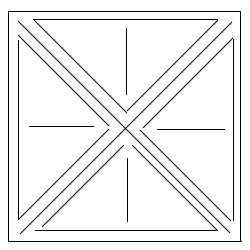
\includegraphics[width=0.7\linewidth]{figures/platzhalter}
  	\caption[kurze Unter-Überschrift]{lange Unter-Überschrift}
  	\label{fig:platzhalter}
  \end{figure}
  In section \ref{sec:PlaneProbDef} the plane's functional was derived. Now the focus is on the functional's discretization. Figure \ref{fig:platzhalter} shows a general, planar object defined to be placed in the xy-plane. The first discretization step is to divide the object into single triangles approximating the shape of it. This process is called triangulation. Every one of these triangles then represents a finite element with one node at every corner. The finer the triangulation is done the better the object and its boundary are matched by its discrete complement, but also the more finite elements have to be considered in later calculations.
  \begin{figure}
  	\centering
  	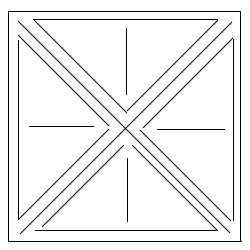
\includegraphics[width=0.7\linewidth]{figures/platzhalter}
  	\caption[kurze Unter-Überschrift]{lange Unter-Überschrift}
  	\label{fig:platzhalter}
  \end{figure}
  One triangular finite element is shown in Figure \ref{fig:platzhalter}. It is defined by the coordinates $(x_i,y_i)$ of its three nodes. Since the element is located in the xy-plane, the z-coordinate is of no interest and will be ignored. At every node, forces can be applied denoted with $F_{x_i}$ and $F_{y_i}$. Accordingly, every node can be displaced. The movement along the x-axis is denoted with $u_i$, or with $v_i$ along the y-axis respectively. Note, that the node numbering is in counter-clockwise direction. This definition will be kept throughout the thesis, and is important to remember when implementing the FEM-code in order to reduce errors.
  In this thesis only triangles defined by three nodes are discussed. There are many more finite elements forming triangles, such as six node triangles or even seven node triangles. The main difference between these types of elements are the order of shape functions. More details about higher order triangular finite elements can be found in %TODO \cite
  
  % ansatzfunktion (abgewandelt statt phi, u und v separat)\\
  In the case of a three node triangle the basis functions for the two displacements $u$ and $v$ are as follows \cite{steinke2005finite}:
  \begin{equation}\label{eq:t3_ansatzU}
  u(x,y) = a_0 + a_1L_1 + a_2L_2 = \begin{pmatrix}
  1 & L_1 & L_2
  \end{pmatrix} \begin{pmatrix}
  a_0 \\ a_1 \\ a_2
  \end{pmatrix} = \vec{x}^T \vec{a},
  \end{equation}
  \begin{equation}\label{eq:t3_ansatzV}
  v(x,y) = a_0 + a_1L_1 + a_2L_2 = \begin{pmatrix}
  1 & L_1 & L_2
  \end{pmatrix} \begin{pmatrix}
  a_0 \\ a_1 \\ a_2
  \end{pmatrix} = \vec{x}^T \vec{a},
  \end{equation}
  both defined in trilinear coordinates (see figure \ref{fig:platzhalter}).
  % dreieckskoordinaten (ähnlich bild 2.7 auf s.39(53))
  \begin{figure}
  	\centering
  	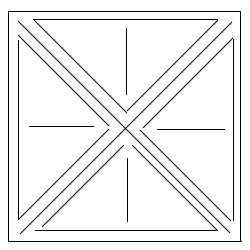
\includegraphics[width=0.7\linewidth]{figures/platzhalter}
  	\caption[kurze Unter-Überschrift]{lange Unter-Überschrift}
  	\label{fig:platzhalter}
  \end{figure}
  % interpolationsbedingunen führen auf Formfunktionen\\
  To get the unknown coefficients $a_i$, values for the trilinear coordinates are set. This creates a system of linear equations:
  \begin{align}
  u(L_1=1, L_2=0) = u_1 &\rightarrow u_1 = a_0 + a_1 \nonumber\\
  u(L_1=0, L_2=1) = u_2 &\rightarrow u_2 = a_0 + a_2 \nonumber\\
  u(L_1=0, L_2=0) = u_3 &\rightarrow u_3 = a_0
  \end{align}
  Alternatively, this could be also done with $v$. Written as matrix and vector:
  \begin{align}
  \underline{A} \vec{a} = \vec{u} \nonumber\\
  \begin{pmatrix}
  1 & 1 & 0\\
  1 & 0 & 1\\
  1 & 0 & 0
  \end{pmatrix} \begin{pmatrix}
  a_0 \\ a_1 \\ a_2
  \end{pmatrix} = \begin{pmatrix}
  u_1 \\ u_2 \\ u_3
  \end{pmatrix}
  \end{align}
  Now, inverting matrix $A$ the coefficients can be found:
  \begin{equation}\label{eq:t3_coeffsA}
  \vec{a} = \underline{A}^{-1} \vec{u} = \begin{pmatrix}
  0 & 0 & 1\\
  1 & 0 & -1\\
  0 & 1 & -1
  \end{pmatrix} \begin{pmatrix}
  u_1 \\ u_2 \\ u_3
  \end{pmatrix}
  \end{equation}
  If one put equation \ref{eq:t3_coeffsA} into \ref{eq:t3_ansatzU}, or the analogon into \ref{eq:t3_ansatzV}, the shape functions for the three node triangular finite element will be derived, as described in \cite{steinke2005finite}:
  \begin{align}\label{eq:t3SF}
  u &= \vec{x}^T \vec{a} = \vec{x}^T \underline{A}^{-1}\vec{u} = \vec{N}^T\vec{u} \nonumber\\
  \vec{N}^T &= \vec{x}^T \underline{A}^{-1} =
  \begin{pmatrix}
  1 & L_1 & L_2
  \end{pmatrix} \begin{pmatrix}
  0 & 0 & 1\\
  1 & 0 & -1\\
  0 & 1 & -1
  \end{pmatrix} \nonumber\\
  &= \begin{pmatrix}
  L_1 & L_2 & 1-L_1-L_2
  \end{pmatrix} = \begin{pmatrix}
  N_1 & N_2 & N_3
  \end{pmatrix}
  \end{align}
  Characteristically for the shape function, as stated in \cite{steinke2005finite}, is, that shape function $N_i$ gets the value 1 at node $i$ and 0 at the two other nodes. The functions are linear with respect to $L_1$ and $L_2$ which can be noticed in equation \ref{eq:t3SF}. As stated before, these shape functions are the same for displacement $u$ and $v$. With the knowledge of the displacement values of the element's nodes one can formulate the displacement functions in trilinear coordinate notation as follows:
  \begin{align}
  u &= N_1 u_1 + N_2 u_2 + N_3 u_3 \nonumber\\
  v &= N_1 v_1 + N_2 v_2 + N_3 v_3
  \end{align}
  Or in matrix form:
  \begin{align}
  \vec{\hat{u}} &= \underline{N} \vec{u} \nonumber\\
  \begin{pmatrix}
  u \\ v
  \end{pmatrix} &= \begin{pmatrix}
  N_1 & 0 & N_2 & 0 & N_3 & 0 \\
  0 & N_1 & 0 & N_2 & 0 & N_3
  \end{pmatrix} \begin{pmatrix}
  u_1 \\ v_1 \\ u_2 \\ v_2 \\ u_3 \\ v_3
  \end{pmatrix}
  \end{align}
  % Dehnungs-Verschiebungs-Beziehung -> führt zu B + Spannungs-Verschiebungs-Beziehung\\
  % Einsetzen in Gesamtpotential + Variation\\
  % Bestimmung von K kürzen: wichtig ist nur s.221 K = t*int(H*dA,A) mit dV = t*dA
  \subsubsection{Quad-4 Plane Element}
  - mathematical derivation of four node quadrilateral plane element\newline
  - see Steinke \cite{steinke2005finite} page 237-250 + Cook \cite{cook2002concepts} page 202-208\\
  - isoparametrisches viereckselement (7.5.1) + bild\\
  - bild von original- und bildebene\\
  - eigenschaften der ansatzfunktion + formfunktionen\\
  - verschiebungen von uv mit formfunktionen und u darstellen\\
  - jacobi-matrix aufstellen, inverse und determinante nicht so genau (bzw. einfach, weil J eh nur 2x2 ist)\\
  - dehnungs-verschiebungs-beziehung AUS ANDERER QUELLE, DA IN \cite{steinke2005finite} UNZUFRIEDENSTELLEND BESCHRIEBEN\\
  - stefigkeitsmatrix $K = int_V(B^TDBdV) = t*int_V(B^TDBdA) = t*int_-1^1 int_-1^1(B^TDB|J|dsdr)$ + erwähnen, dass |J| Flächeninhalt angibt (ref finden)
 \subsection{Plate Bending Element}
 Second part of shell element: plate part. derivation of this part with two exemplary finite element types
  \subsubsection{Problem Definition}
  \cite{steinke2005finite} ch8.1\\
  - bild wie bei \ref{sec:MprobDef}\\
  - hier wird die kirchhoff-platten-theorie verwendet\\
  - voraussetzungen der kirchhoff-platte\\
  - größen der platte: durchbiegung w + verdrehungen dw/dx bzw. dw/dy\\
  - dehnungs-verschiebungs-beziehung\\
  - stoffgleichung (krümmungs-momenten-beziehung) -> führt auf Dp und Querkräfte Qx,Qy\\
  - gleichgewichtsbeziehung der platte (p ist flächenlast; näher untersuchen)\\
  - auf verschiedene randbedingungen der platte eingehen\\
  - funktional der platte\\
  - forderungen an plattenelement
  \subsubsection{Tri-3 Plate Element} \cite{steinke2005finite}\cite{specht1988modified}
  - mathematical derivation of three node triangular plane element\newline
  - see Steinke \cite{steinke2005finite} page 275-282 + \cite{specht1988modified} for reference of element\\
  - 8.4.4 beschreibt probleme mit einigen dreiecksplattenelementen, deshalb für meine arbeit element von specht \cite{specht1988modified}\\
  - ansatzfunktion nach specht\\
  - interpolationsbedingungen\\
  - entwicklung der formfunktionen\\
  - krümmungs-verschiebungs-beziehung\\
  - steifigkeitsmatrix
  \subsubsection{Quad-4 Plate Element}
  - mathematical derivation of four node quadrilateral plane element\newline
  - see Zienkiewicz \cite{zienkiewicz2000finite} page 174-177,219-222  \cite{zienkiewicz1977fem} ???  \textbf{\cite{batoz1982evaluation} page 1658-1662}\\
  - formulierung als DKQ element\\
  - \textbf{!! formatierung an meine anpassen, da sehr unterschiedlich zu anderen referenzen !!}\\
  - dkq basiert auf diskretisierung der stress-energie, unter vernachlässigung der transverse shear strain energy (gl.(1) s.4)\\
  - krümmungsvektor, Db angeben\\
  - considerations für dkq formulierung\\
  - formfunktionen, koeffizienten\\
  - jacobi-matrix, -inverse, determinante\\
  - krümmungs-verschiebungs-beziehung\\
  - steifigkeitsmatrix
 \subsection{Coordinate Transformation} %\cite{steinke}
 \textit{erster Entwurf}\newline
 see \cite{nguyen2008smoothed}; genau: \cite{zienkiewicz2000finite}\\
 The nodes and elements in the mesh are defined in global three dimensional space. The elements need to be transformed into local two dimensional space in order to be able to calculate their local stiffness matrix. This local stiffness matrix must then be transformed back into the global system.
 Transform arbitrary 3D triangle onto xy-Plane:
 % Bild von Dreieck mit ABC, globalem KoSys, lokalem KoSys mit Ursprung in A, x-Achse auf Vektor AB usw.\newline
 - given triangle with vertices $A=(a_x, a_y, a_z), B=(b_x, b_y, b_z)$ and $C=(c_x, c_y, c_z)$ ordered in counter-clockwise direction\newline
 - let $U$ be the vector from node $A$ to $B$: $U = B-A = (b_x-a_x, b_y-a_y,b_z-a_z)$ and let $V$ be the vector from node $A$ to $C$: $V = C-A = (c_x-a_x,c_y-a_y,c_z-a_z)$\newline
 - First local unit vector $\tilde{x} = \frac{1}{\left|U\right|}U$\newline
 - Second local unit vector $\tilde{z} = U \times V \longrightarrow \tilde{z} = \frac{1}{\tilde{z}}\tilde{z}$\newline
 - Third local unit vector $\tilde{y} = \tilde{z} \times \tilde{x}$\newline
 - Define transformation matrix $T$ as follows: \[T = \begin{pmatrix}
 \tilde{x}^T\\ \tilde{y}^T\\ \tilde{z}^T
 \end{pmatrix}
 = \begin{pmatrix}
  \tilde{x}_x & \tilde{x}_y & \tilde{x}_z\\ \tilde{y}_x & \tilde{y}_y & \tilde{y}_z\\ \tilde{z}_x & \tilde{z}_y & \tilde{z}_z
  \end{pmatrix}\]
  - Assembly of element's stiffness needs derivatives. Therefore every triangle can be translated in such a way, that node $A$ lies in the global origin.\newline
  - It follows: $\tilde{A} = \left(0\ 0\ 0\right)^T, \tilde{B} = \left(\tilde{b}_x\ 0\ 0\right)^T, \tilde{C} = \left(\tilde{c}_x\ \tilde{c}_y\ 0\right)^T$\newline
  - Node $A$ will not be changed by the transformation with $T$, $B$ will be projected onto the local x-axis due to the definition of it as the vector between $A$ and $B$ and $C$ will be projected onto the local $xy$-plane.\newline
  - One can see that the z component vanishes by transforming into local space\newline
  \newline
  % Bild von bel. Viereck mit ABCD, IJKL, globalem KoSys, lokalem KoSys mit Ursprung auf Schnittpunkt der gestrichelten Linien von JL und IK\newline
  - given quadrilateral with vertices $A=(a_x, a_y, a_z), B=(b_x,b_y,b_z), C=(c_x,c_y,c_z), D=(d_x,d_y,d_z)$ ordered in counter-clockwise direction\newline
  - let $I$ be the midpoint of the edge $AB$ as follows: $I = A+\frac{1}{2}(B-A)$. Analogously let $J$,$K$ and $L$ be the midpoints of the edges $BC$, $CD$ and $DA$: $J = B+\frac{1}{2}(C-B), K = C+\frac{1}{2}(D-C), L = D+\frac{1}{2}(A-D)$\newline
  - let $U$ be the vector from node $L$ to $J$: $U = J-L = (j_x-l_x,j_y-l_y,j_z-l_z)$ and let $V$ be the vector from node $I$ to $K$: $V = K-I = (k_x-i_x,k_y-i_y,k_z-i_z)$\newline
  - First local unit vector $\tilde{x} = \frac{1}{\left\|U\right|}U$\newline
  - Second local unit vector $\tilde{z} = U \times V \longrightarrow \tilde{z} = \frac{1}{\left|\tilde{z}\right|}\tilde{z}$\newline
  - Third local unit vector $\tilde{y} = \tilde{z} \times \tilde{x}$\newline
  - Define transformation matrix $T$ as follows: \[T = \begin{pmatrix}
   \tilde{x}^T\\ \tilde{y}^T\\ \tilde{z}^T
   \end{pmatrix}
   = \begin{pmatrix}
    \tilde{x}_x & \tilde{x}_y & \tilde{x}_z\\ \tilde{y}_x & \tilde{y}_y & \tilde{y}_z\\ \tilde{z}_x & \tilde{z}_y & \tilde{z}_z
    \end{pmatrix}
    \]
 \subsection{Shell Element}
 The combination of the two previous parts and the transformations results in the final shell element\newline
 - bild wie bei 8.7 von scheibe und platte und kombination zu schale + erklärungen, welche unbekannten und kräfte man bei welchem teil hat\\
 - erklärung, warum man hier einfach Plane und Plate unabhängig voneinander berechnen und dann zusammenwerfen darf\\
 - gesamtsteifigkeitsmatrix besteht aus blöcken (3x3 bei tri3, 4x4 bei quad4), Ku=F (gleichung 718 bei \cite{steinke2005finite})
 - Sei $K_m$ die lokale Steifigkeitsmatrix vom Membran/Plane-Teil und $K_p$ die vom Plate-bending-Teil\\
 - Kij weisst in der Spalte theta\_z und Zeile theta\_z $(k_ij)_66$ eine null auf -> erklärung und warum schlecht. ANDERE REFERENZ ERKLÄRT, WAS WIR DESHALB MACHEN (1/1000 der diagonalwerte)\\
 - Dann muss die (Rück-)Transformationsmatrix $T$ erstellt werden, da SKM im lokalen KoSys definiert ist, aber in die globale Systemmatrix einsortiert werden muss\\
 - Je nachdem ob 3 oder 4 Knotenelement (Tri-3/Quad-4) sieht $K$ und $T$ natürlich anders aus\newline
 - Wir transformieren blockweise von lokal nach global zurück ($K_{ij}, 1 \leq i,j \leq 3(4)$)\newline
 \newpage
\section{FEM Code Implementation}
contains development of the program code with focus on the assembly of the system and its solving, the process of parallelization and the coupling step with preCISE
 \subsection{Introduction to libMesh}
 was kann libMesh eigentlich alles; wo unterstützt es einen, was muss man selbst machen
 \subsection{libMesh FEM}
 details about the implementation with the libmesh FEM framework:\newline
 - initialization: loading of parameters, setting up libmesh (evtl. uninteressant und es kann weg, oder es muss noch mehr hier rein)\newline
 - mesh loading/import: wie sieht mesh file aus bzw. welche typen werden akzeptiert, welche ids für bcs müssen verwendet werden\newline
 - set up of system: erstellen des linearimplicitsystems, erstellen der variablen, der bcs, des solvers usw.\newline
 - assembly of system matrix and RHS: größter teil; hier wird auf die erstellung der lokalen und globalen stiffnessmatrix eingegangen (integral mit gauss-quadratur lösen z.B. \cite{steinke2005finite} s.248), das auslesen der forces und der entsprechende eintrag in der rhs gesetzt; das mitverfolgen der bereits bearbeiteten knoten mittels unordered\_set usw.\newline
 - boundary conditions: eventuell bereits unter setup; grundsätzlich auf die beiden bc-typen eingehen, wie das in libmesh gelöst wurde\newline
 - solving and getting the result vector: das lösen an sich ist eine code-zeile. hier kann man aber schreiben, mit was libmesh umgehen kann an lösern, welche einstellmöglichkeiten es gibt (error-eps, \#iters). und es geht drum, wie man an die tatsächlichen werte für die displacements kommt und was daraus am ende wird\newline
 - für die standalone-version noch ein absatz zur ausgabe in exodus2-file
 \subsection{Parallelization with MPI}
 additional steps to make the code ready for multi process execution with MPI\newline
 - viel ist es nicht, was man tun muss, damit libmesh mit mpi läuft\newline
 - grundsätzlich ist zum lösen des gleichungssystem mit mehreren prozessen petsc als externe lib notwendig\newline
 - am mesh muss nichts verändert werden, da libmesh automatisch eine partitionierung des meshes vornimmt (kann aber verbessert werden)\newline
 - damit rhs korrekt gesetzt wird muss über die prozessgrenzen hinweg klar sein, ob knoten bereits bearbeitet wurde oder nicht. wie das gelöst wurde kommt hier rein\newline
\section{Coupling with preCICE}
still under construction; just a rough idea what this section will contain
 \subsection{Coupling}
 short introduction what coupling means (in this case)
  \subsubsection{Introduction to coupling}
  $\dots$
  \subsubsection{Coupling methods}
  $\dots$
 \subsection{preCICE}
 short introduction what preCICE is
 \subsection{Implementation}
 "modification" of the code to work with preCICE
\newpage
\section{Validation}
The code was tested with several problems to validate its correctness and state where and why there are differing results to the existing (commercial) FEM codes
 \subsection{Test A: Membrane Displacement with Tri-3}
 Sprungbrett bestehend aus 8 Elementen; links fest eingespannt, rechts Kraft in y-Richtung an beiden Randknoten\newline
 Sprungbrett bestehend aus 32 Elementen in Fischgrätmuster angeordnet; selbe BCs aber andere Kraftwerte\newline
 test\_c.xda, test\_d.xda - beides korrekt
 \subsection{Test B: Membrane Displacement with Quad-4}
 Sprungbrett bestehend aus 3 Elementen mit BC wie in Test A aber einzelne Kraft auf oberen rechten Knoten in neg. y-Richtung\newline
 selbes Mesh wie in test\_d.xda nur eben mit 16 Elementen. Selbe BCs, selbe Kraftwerte\newline
 test\_e.xda, test\_f.xda - beides korrekt
 \subsection{Test C: Plate Displacement with Tri-3}
 Platte an allen 4 Seiten eingespannt. Einzelne Kraft im Zentrum in neg. z-Richtung\newline
 Alternativ mit anderen Parametern test\_g\newline
 test\_a\_triN.xda, test\_g\_triAB\_N.xda - korrekt, noch nicht getestet
 \subsection{Test D: Plate Displacement with Quad-4}
 Selbes mesh wie Test C nur eben mit Quadelementen\newline
 test\_a\_quadN.xda, test\_g\_quad\_N.xda - korrekt, noch nicht getestet
 \subsection{Test E: Shell Displacement with Tri-3}
 Ein H-Trägerbalken. Am einen Ende fest eingespannt. Am anderen Ende wird oben eine Kraft am äußeren Knoten in den Balken hinein in flacher Ebene gegeben, gleichzeitig wird unten an der gegenüberliegenden Seite eine Kraft in entgegengesetzter Richtung gegeben\newline
 test\_j\_tri.xda - korrekt
 \subsection{Test F: Shell Displacement with Quad-4}
 Gleich wie Test E nur eben Quadelemente\newline
 test\_j\_quad.xda - korrekt
 \subsection{Test G: Convergence (increasing number of elements)}
 ??? theoretisch mit Test C/D bereits durchführbar mit N=2,4,8,16,32,64,128
 \subsection{Test H: MPI (increasing number of processes)}
 ??? theoretisch alle Tests, z.B. E/F mit Prozessoranzahl = 1,2,4,8,16. In dem Fall ist natürlich die Zeit interessant und ob die Ergebnisse jeweils alle gleich sind
 \subsection{Test I: Coupling with preCICE}
 ???
% \subsection{Test J: Time dependence + mass matrix and damping matrix}
% ???
\newpage
\section{Conclusion}
What does my code do, what problems arose, what problems persist, what does my code cannot do, where are opportunities for extensions, etc.
\newpage
\bibliographystyle{alpha}
\bibliography{thesis}
\Affirmation
\end{document}